% -*- latex -*-
%%%%%%%%%%%%%%%%%%%%%%%%%%%%%%%%%%%%%%%%%%%%%%%%%%%%%%%%%%%%%%%%
%%%%%%%%%%%%%%%%%%%%%%%%%%%%%%%%%%%%%%%%%%%%%%%%%%%%%%%%%%%%%%%%
%%%%
%%%% This text file is part of the source of 
%%%% `Introduction to High-Performance Scientific Computing'
%%%% by Victor Eijkhout, copyright 2012-6
%%%%
%%%% This book is distributed under a Creative Commons Attribution 3.0
%%%% Unported (CC BY 3.0) license and made possible by funding from
%%%% The Saylor Foundation \url{http://www.saylor.org}.
%%%%
%%%%
%%%%%%%%%%%%%%%%%%%%%%%%%%%%%%%%%%%%%%%%%%%%%%%%%%%%%%%%%%%%%%%%
%%%%%%%%%%%%%%%%%%%%%%%%%%%%%%%%%%%%%%%%%%%%%%%%%%%%%%%%%%%%%%%%

\index{nested dissection ordering|(}
\index{matrix ordering!nested dissection|see{nested dissection ordering}}

Above, you have seen several examples of ordering the variables in the
domain other than with the \indexterm{lexicographic ordering}. In this
section you will see the \emph{nested dissection ordering}, which was
initially designed as a way to reduce fill-in. However, it is also
advantageous in a parallel computing context.

Nested dissection is a recursive process for determining a nontrivial
ordering of the unknowns in a domain. In the first step, the
computational domain is split in two parts, with a dividing strip
between them; see figure~\ref{fig:domdecomp}.
\begin{figure}[ht]
  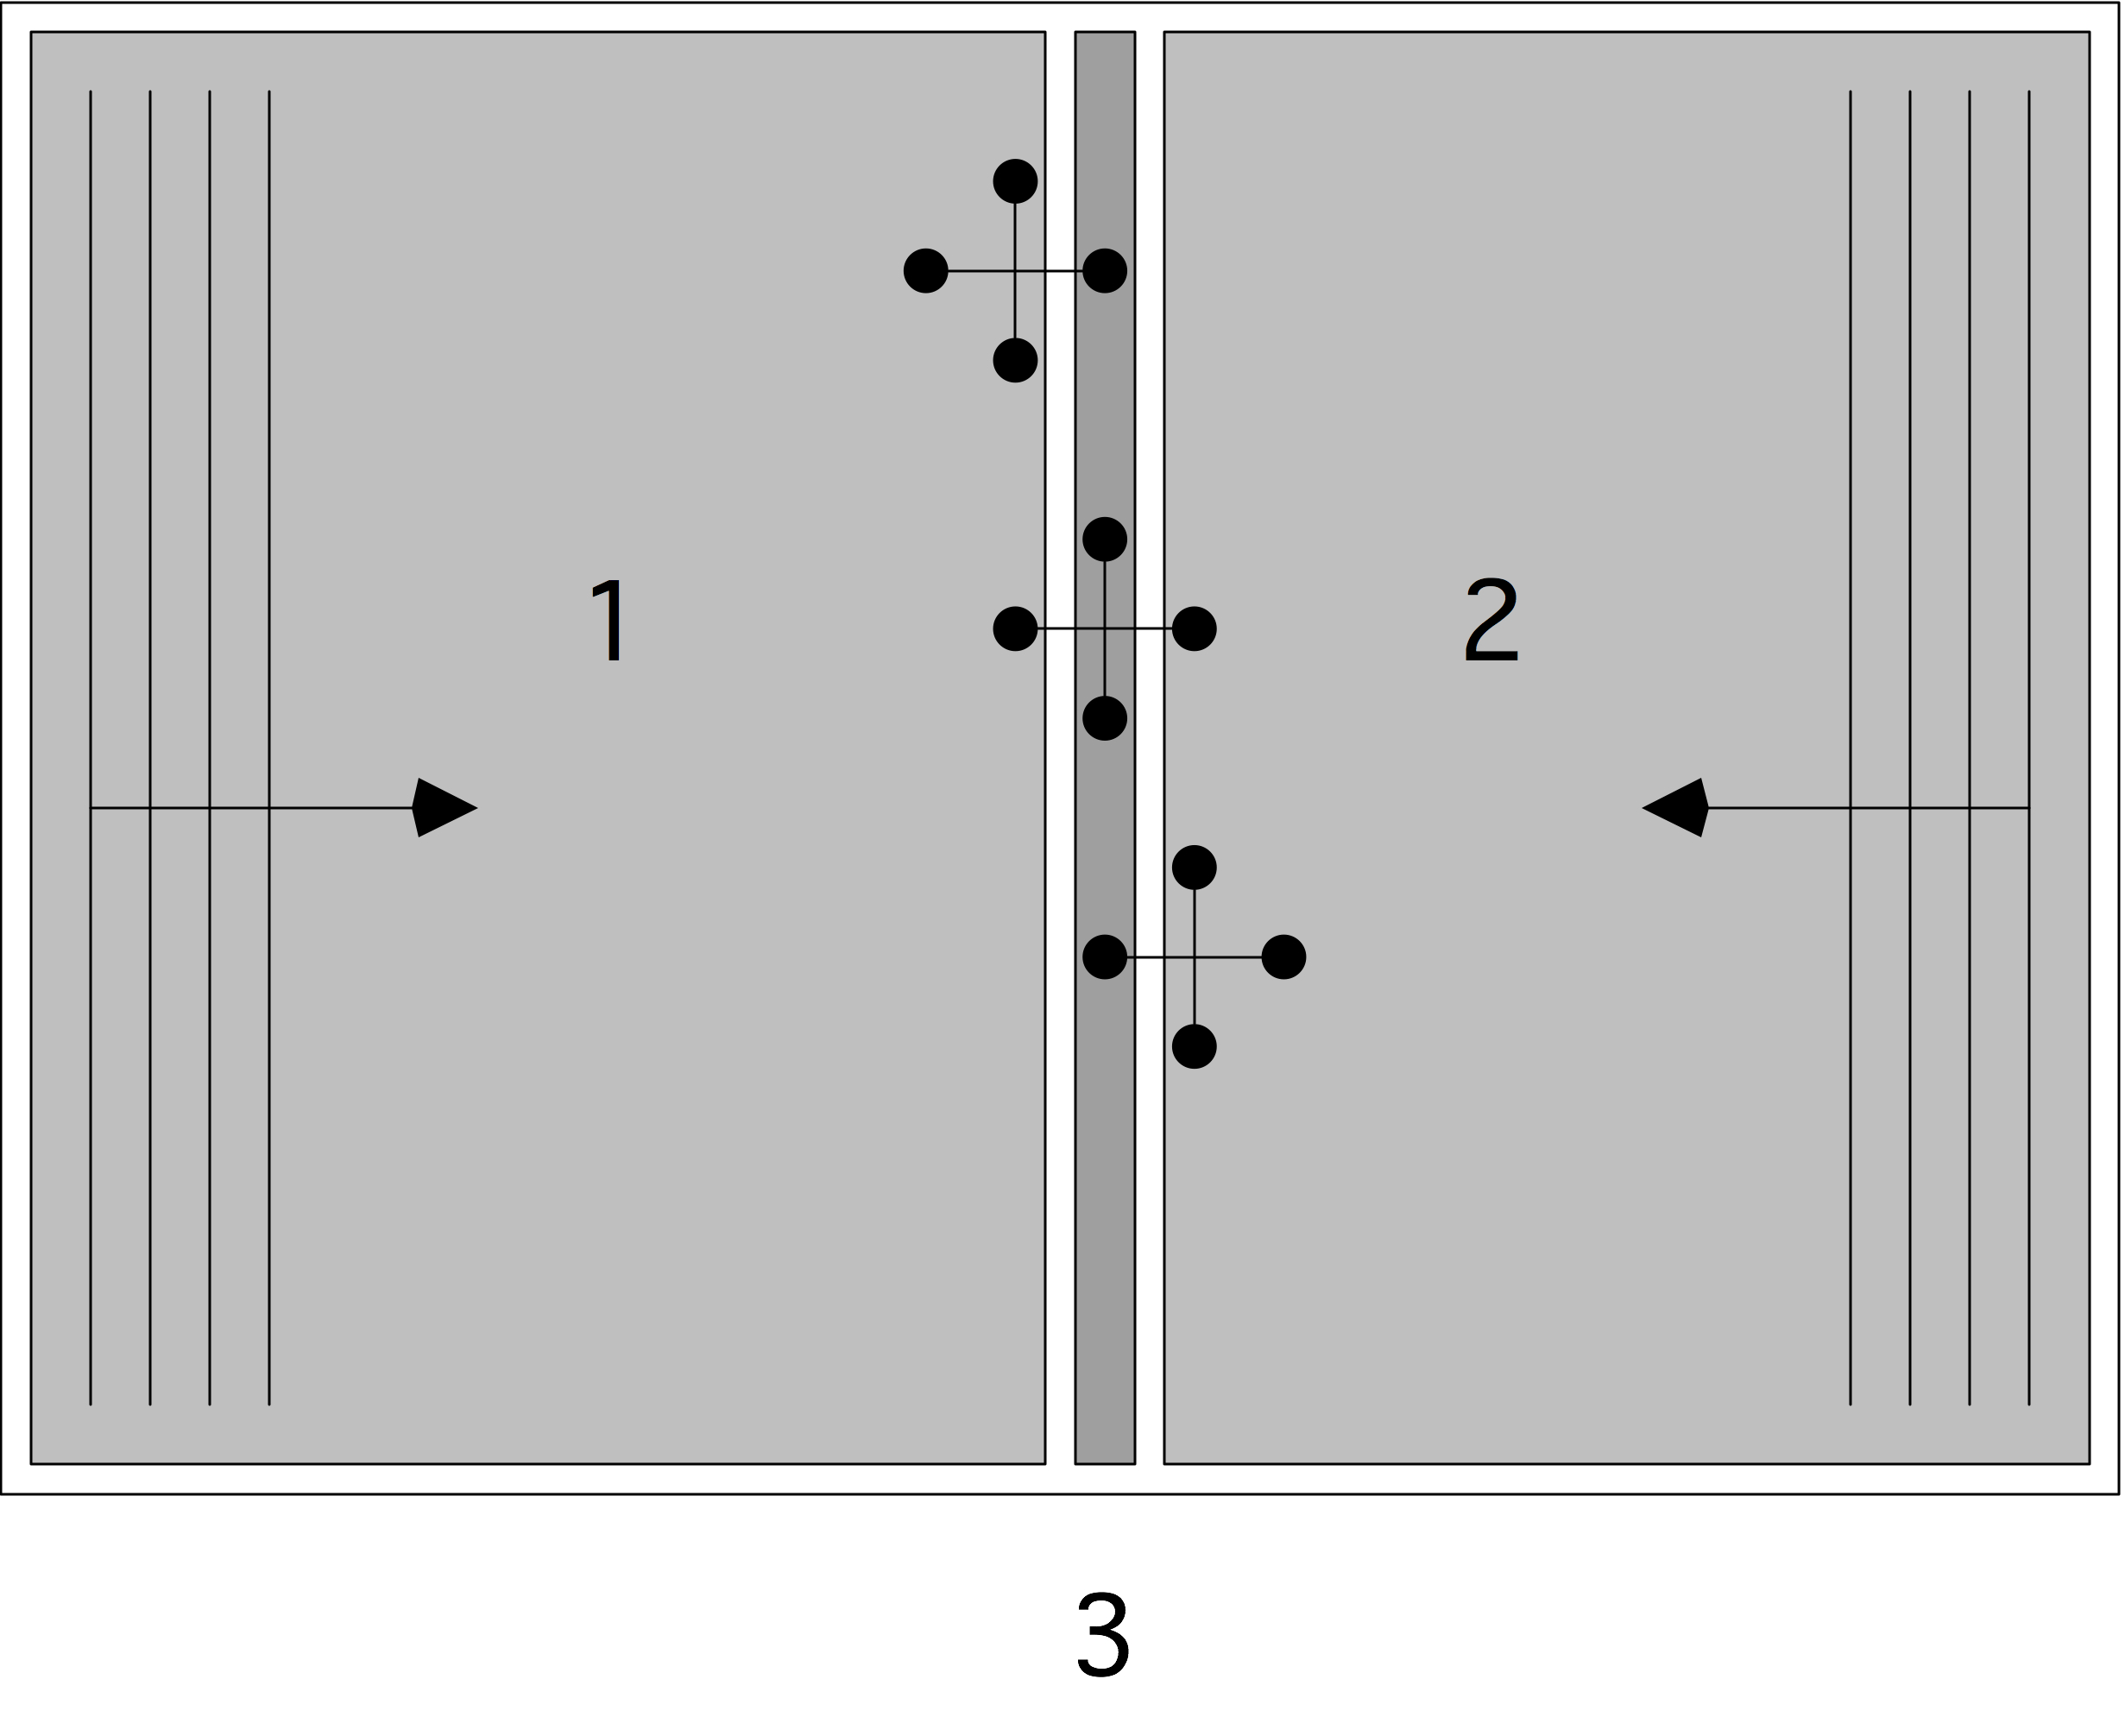
\includegraphics[scale=.1]{graphics/domdecomp}
  \caption{Domain dissection into two unconnected subdomains and a separator}
  \label{fig:domdecomp}
\end{figure}
\newcommand\Add{A^{\mathrm{DD}}}
To be precise, the \indexterm{separator} is wide enough that there are
no connections between the left and right \indexterm{subdomain}. The resulting
matrix $\Add$ has a $3\times3$ structure, corresponding to the three
divisions of the domain. Since the subdomains $\Omega_1$
and~$\Omega_2$ are not connected, the submatrices $\Add_{12}$
and~$\Add_{21}$ are zero.
\[
  \Add=
  \begin{pmatrix}
    A_{11}&\emptyset&A_{13}\\
    \emptyset&A_{22}&A_{23}\\
    A_{31}&A_{32}&A_{33}
  \end{pmatrix}=
\left(\begin{array}{ccccc|ccccc|c}
  \star&\star &      &      &      &&&&&&0\\
  \star&\star &\star &      &      &&&&&&\vdots\\
       &\ddots&\ddots&\ddots&      &&&\emptyset&&&\vdots\\
       &      &\star &\star &\star &&&&&&0\\
       &      &      &\star &\star &&&&&&\star\\ \hline
  &&&&&\star&\star &      &      &      &0\\
  &&&&&\star&\star &\star &      &      &\vdots\\
  &&\emptyset&&&     &\ddots&\ddots&\ddots&      &\vdots\\
  &&&&&     &      &\star &\star &\star &0\\
  &&&&&     &      &      &\star &\star &\star\\ \hline
  0&\cdots&\cdots&0&\star&0&\cdots&\cdots&0&\star&\star
\end{array}\right)
\begin{array}{c}
  \left.\begin{array}{c}
    \phantom{0}\\ \phantom{\vdots}\\ \phantom{\vdots}\\ \phantom{0}\\ 
    \phantom{\star}\\
  \end{array}\right\} \\
  \left.\begin{array}{c}
    \phantom{0}\\ \phantom{\vdots}\\ \phantom{\vdots}\\ \phantom{0}\\ 
    \phantom{\star}\\
  \end{array}\right\} \\
  \left.\begin{array}{c}
    \phantom{0}\\ 
  \end{array}\right\}
\end{array}
\begin{array}{c}
  \phantom{0}\\ \phantom{\vdots}\\ (n^2-n)/2\\ \phantom{0}\\ \phantom{\star}\\
  \phantom{0}\\ \phantom{\vdots}\\ (n^2-n)/2\\ \phantom{0}\\ \phantom{\star}\\
  n
\end{array}
\]
This process of dividing the domain by a separator is also called
\indexterm{domain decomposition} or \indexterm{substructuring},
although this name is also associated with the mathematical analysis
of the resulting matrices~\cite{BGSm:96}. In this example of a
rectangular domain it is of course trivial to find a
separator. However, for the type of equations we get from \acp{BVP} it
is usually feasible to find a separator
efficiently for any domain~\cite{LiTa:separator}; 
see also section~\ref{sec:fiedler-vector}.

Let us now consider the $LU$ factorization of this matrix. If we
factor it in terms of the $3\times 3$ block structure, we get
\[
  \Add=LU=
  \begin{pmatrix}
    I\\
    \emptyset&I\\
    A_{31}A_{11}\inv&A_{32}A_{22}\inv&I
  \end{pmatrix}
  \begin{pmatrix}
    A_{11}&\emptyset&A_{13}\\
         &A_{22}&A_{23}\\
    &&S_{33}
  \end{pmatrix}
\]
where \[ S_{33}=A_{33}-A_{31}A_{11}\inv A_{13}-A_{32}A_{22}\inv A_{23}. \]
The important fact here is that 
\begin{itemize}
\item the contributions $A_{31}A_{11}\inv A_{13}$ and
  $A_{32}A_{22}\inv A_{23}$ can be computed simultaneously, so the
  factorization is largely parallel; and
\item both in the forward and backward solve, components 1 and~2 of
  the solution can be computed simultaneously, so the solution process
  is also largely parallel.
\end{itemize}
The third block can not trivially be handled in parallel, so this
introduces a sequential component in the algorithm. We also need to
take a closer look at the structure of~$S_{33}$.

\begin{exercise}
  In section~\ref{sec:lu-graph} you saw the connection between LU
  factorization and graph theory: eliminating a node leads to a graph
  with that node removed, but with certain new connections added.
  Show that, after eliminating the
  first two sets of variables, the graph of the remaining matrix on
  the separator will be fully connected.
\end{exercise}

The upshot is that after eliminating all the variables in blocks 1
and~2 we are left with a matrix~$S_{33}$ that is fully
dense of size $n\times n$. 

The introduction of a separator gave us a factorization that was
two-way parallel. Now we iterate this process: we put a
separator inside blocks 1 and~2 (see figure~\ref{fig:domdecomp2}),
which gives the following matrix structure:
\begin{figure}[ht]
  \begin{quote}
    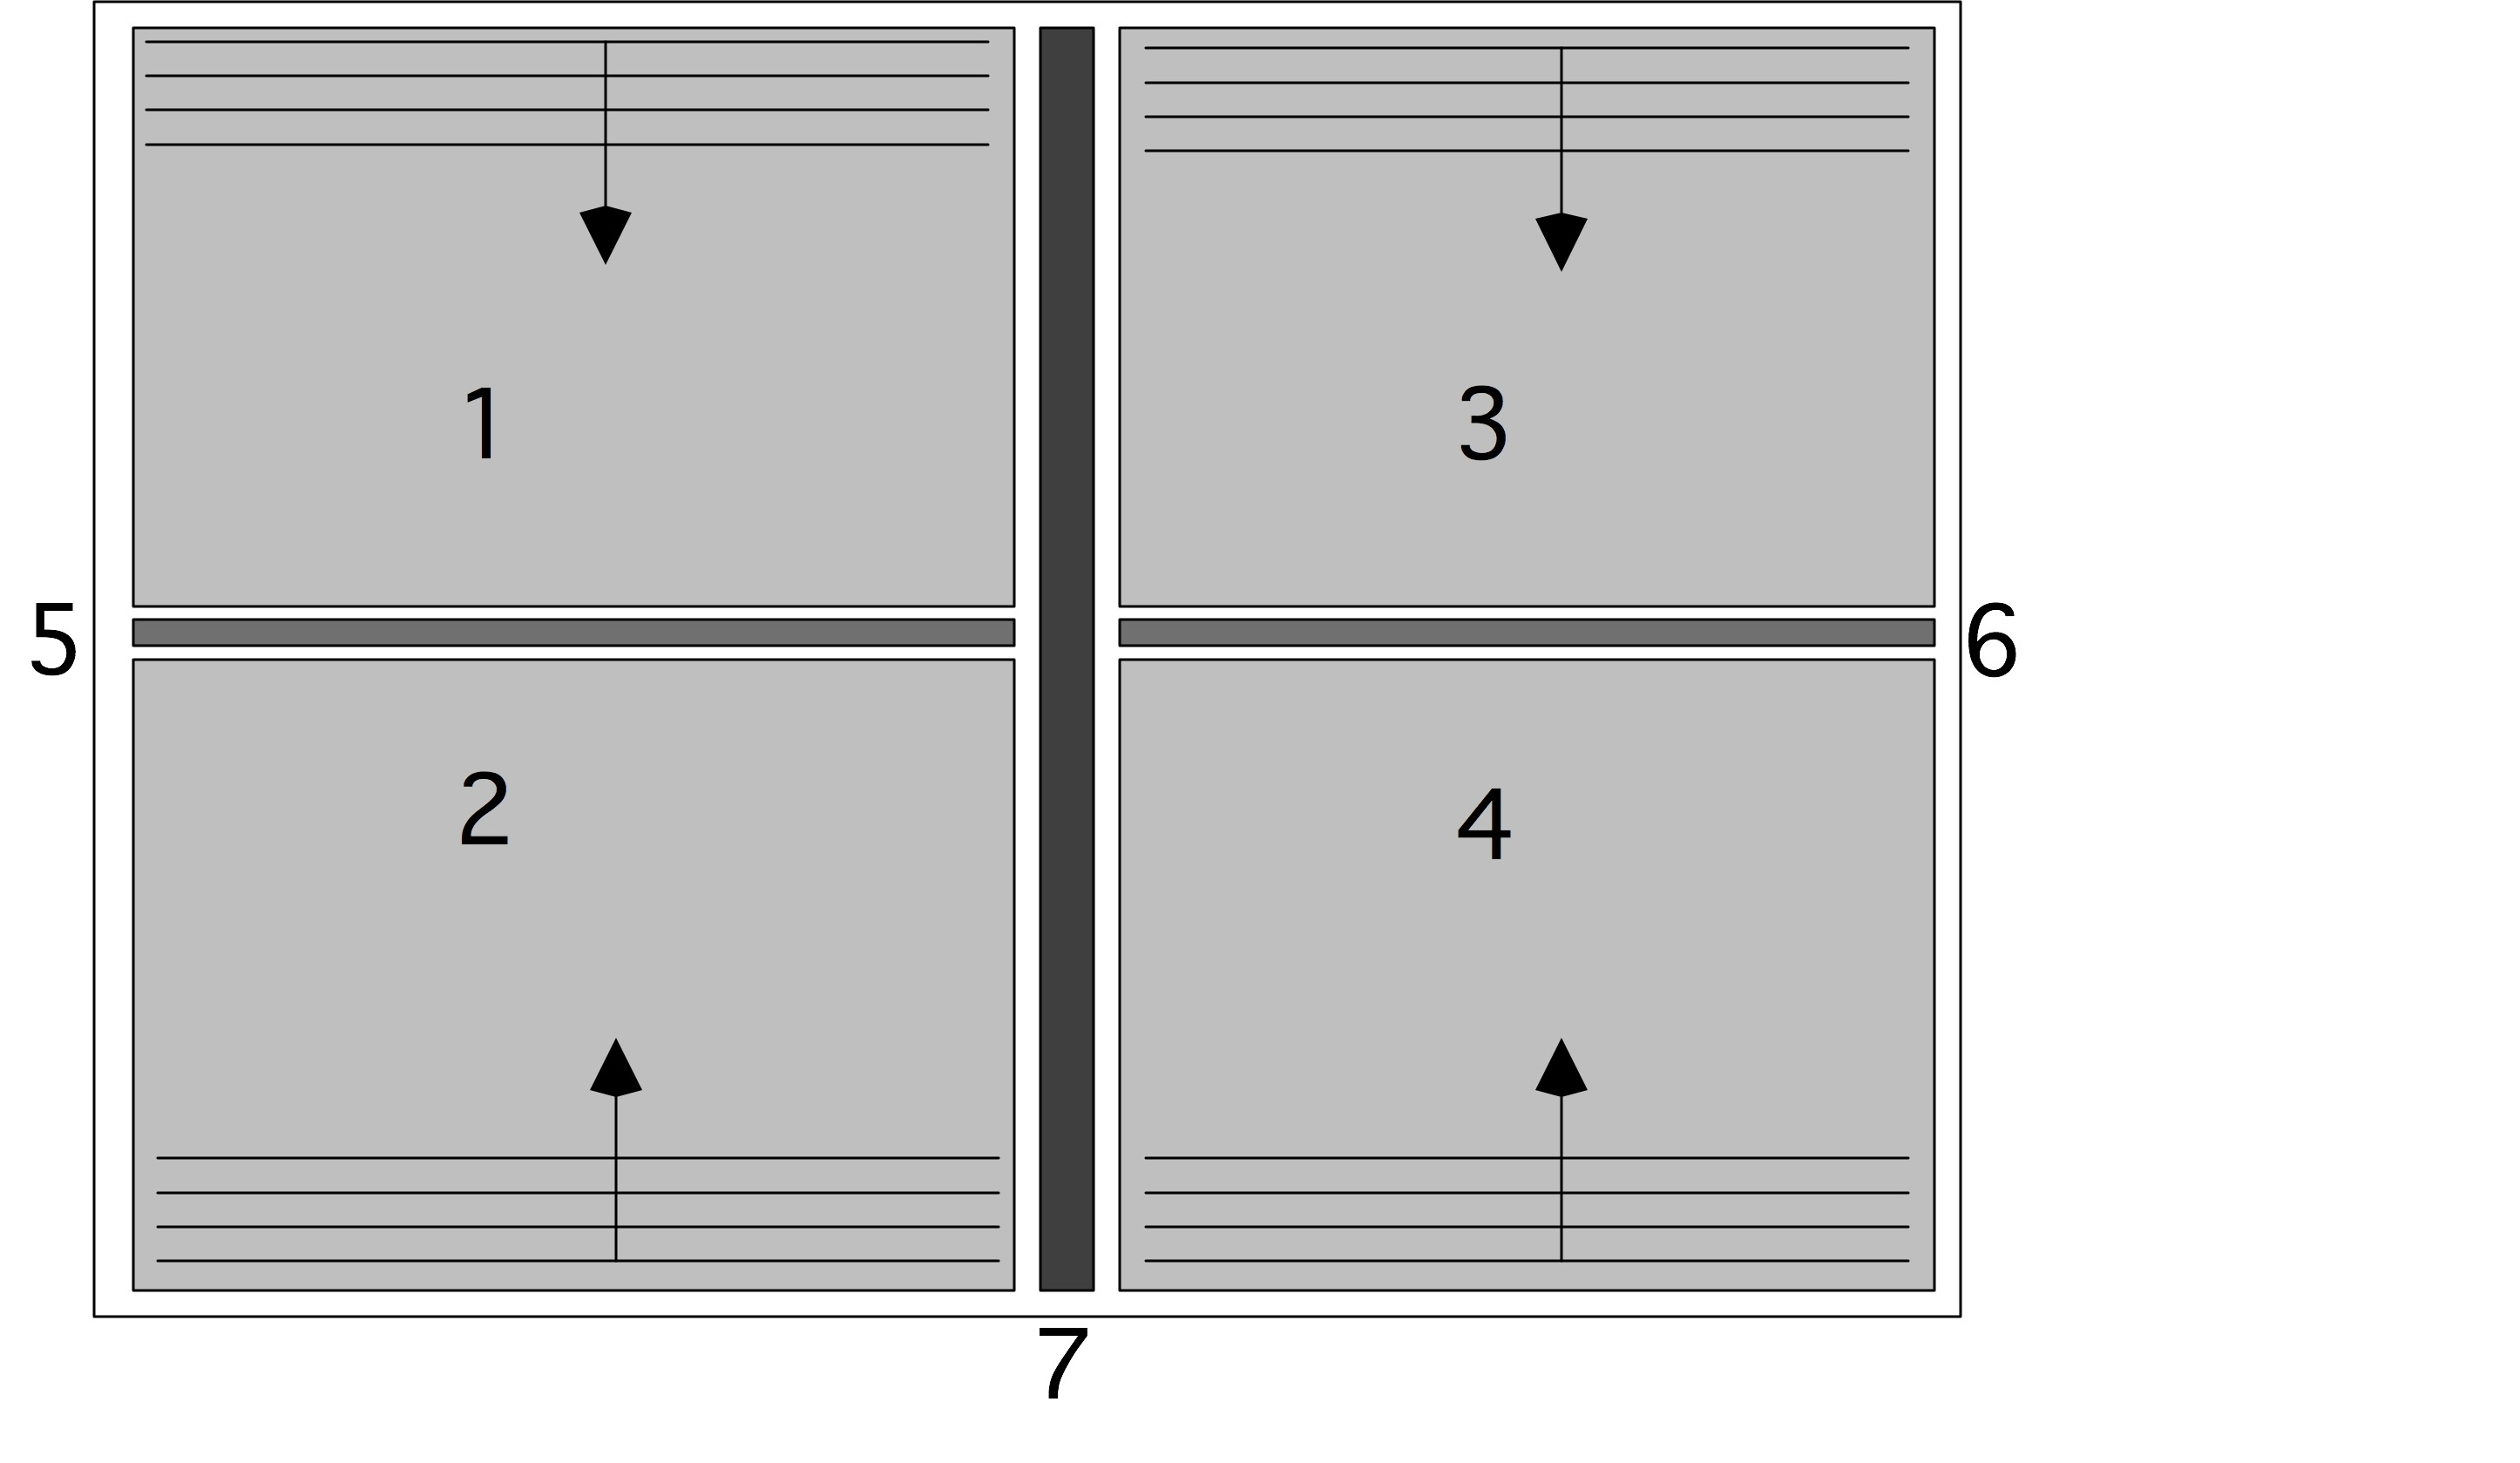
\includegraphics[scale=.11]{graphics/domdecomp2}
  \end{quote}
  \caption{A four-way domain decomposition}
  \label{fig:domdecomp2}
\end{figure}
\[
  \Add=
  \left(\begin{array}{cccc|cc|c}
    A_{11}&     &     &     &A_{15}&     &A_{17}\\
         &A_{22}&     &     &A_{25}&     &A_{27}\\
         &     &A_{33}&     &     &A_{36}&A_{37}\\
         &     &     &A_{44}&     &A_{46}&A_{47}\\ \hline
    A_{51}&A_{52}&    &     &A_{55}&      &A_{57}\\
         &      &A_{63}&A_{64}&    &A_{66}&A_{67}\\ \hline
    A_{71}&A_{72}&A_{73}&A_{74}&A_{75}&A_{76}&A_{77}
  \end{array}\right)
\]
(Note the similarites with the `arrow' matrix in
section~\ref{sec:arrow-matrix}, and recall the argument that this led
to lower fill-in.)
The LU factorization of this is:
\[
  \left(\begin{array}{cccc|cc|c}
        I&     &     &     &      &     &\\
         &I    &     &     &      &     &\\
         &     &I    &     &      &     &\\
         &     &     &I    &      &     &\\ \hline
    A_{51}A_{11}\inv&A_{52}A_{22}\inv&    &     &I    &      &\\
         &      &A_{63}A_{33}\inv&A_{64}A_{44}\inv&   &I     &\\ \hline
    A_{71}A_{11}\inv&A_{72}A_{22}\inv&A_{73}A_{33}\inv&A_{74}A_{44}\inv&
    A_{75}S_5\inv&A_{76}S_6\inv&I
  \end{array}\right) \cdot
\]
\[
  \kern 3\unitindent 
  \left(\begin{array}{cccc|cc|c}
    A_{11}&     &     &     &A_{15}&     &A_{17}\\
         &A_{22}&     &     &A_{25}&     &A_{27}\\
         &     &A_{33}&     &     &A_{36}&A_{37}\\
         &     &     &A_{44}&     &A_{46}&A_{47}\\ \hline
         &     &     &      &S_{5}&      &A_{57}\\
         &     &     &      &     &S_{6} &A_{67}\\ \hline
         &     &     &      &     &      &S_{7}
  \end{array}\right)
\]
where
\[ 
\begin{array}{l}
S_5=A_{55}-A_{51}A_{11}\inv A_{15}-A_{52}A_{22}\inv A_{25},\quad 
   S_6=A_{66}-A_{63}A_{33}\inv A_{36}-A_{64}A_{44}\inv A_{46}\\
   S_7=A_{77}-\sum_{i=1,2,3,4}A_{7i}A_{ii}\inv A_{i7} 
   - \sum_{i=5,6} A_{7i}S_i\inv A_{17}.
\end{array}
\]
Constructing the factorization now goes as follows:
\begin{itemize}
\item Blocks $A_{ii}$ are factored in parallel for $i=1,2,3,4$; similarly
   the contributions $A_{5i}A_{ii}\inv A_{i5}$ for $i=1,2$,
   $A_{6i}A_{ii}\inv A_{i6}$ for $i=3,4$, and $A_{7i}A_{ii}\inv
   A_{i7}$ for $i=1,2,3,4$  can be constructed in parallel.
\item The Schur complement matrices $S_5,S_6$ are formed and
  subsequently factored in parallel, and the contributions
  $A_{7i}S_i\inv A_{17}$ for $i=5,6$ are constructed in parallel.
\item The Schur complement $S_7$ is formed and factored.
\end{itemize}
Analogous to the above reasoning, we
conclude that after eliminating blocks 1,2,3,4 the updated matrices
$S_5,S_6$ are dense of size~$n/2$, and after eliminating blocks 5,6
the Schur complement $S_7$ is dense of size~$n$.

\begin{exercise}
  Show that solving a system with $\Add$ has a similar parallelism to
  constructing the factorization as described above.
\end{exercise}

For future reference, we will call the sets 1 and~2 each others'
siblings, and similarly for 3 and~4. The set 5 is the parent of 1
and~2, 6~is the parent of 3 and~4; 5~and~6 are siblings and 7~is the
parent of 5 and~6.

\Level 2 {Domain decomposition}

In figure \ref{fig:domdecomp2} we divided the domain four ways by a
recursive process. This leads up to our discussion of nested
dissection. It is also possible to immediately split a domain in any
number of strips, or in a grid of subdomains. As long as the
separators are wide enough, this will give a matrix structure with
many independent subdomains.
As in the above discussion, an LU factorization will be characterized
by
\begin{itemize}
\item parallel processing of the subdomains, both in the factorization
  and $L,U$ solves, and
\item a system to be solved on the separator structure.
\end{itemize}

\begin{figure}[ht]
  
\includegraphics[scale=.16]{graphics/domdecomp4}
  \caption{One-way domain decomposition}
  \label{fig:domdecomp4}
\end{figure}

\begin{exercise}
  The matrix from a two-dimensional \ac{BVP} has a block tridiagonal
  structure. Divide the domain in four strips, that is, using three
  separators (see figure~\ref{fig:domdecomp4}). Note that the
  separators are uncoupled in the original matrix.

  Now sketch the sparsity structure of the resulting system on the
  separators are elimination of the subdomains. Show that the system
  is block tridiagonal.
\end{exercise}

In all the domain splitting schemes we have discussed so far we have
used domains that were rectangular, or `brick' shaped, in more than
two dimensions. All of these arguments are applicable to more general
domains in two or three dimensions, but things like finding a
separator become much harder~\cite{LiRoTa:dissection}, and that holds
even more for the parallel case. See section~\ref{sec:fiedler-vector}
for some introduction to this topic.

\Level 2 {Complexity}

The nested dissection method repeats the above process until the
subdomains are very small.  For a theoretical analysis, we keep
dividing until we have subdomains of size~$1\times1$, but in practice
one could stop at sizes such as~$32$, and use an efficient dense
solver to factor and invert the blocks.

To derive the complexity of the algorithm, we take another look at
figure~\ref{fig:domdecomp2}, and see that
complexity argument, the total space a full recursive nested
dissection factorization needs is the sum of
\begin{itemize}
\item one dense matrix on a separator of size~$n$, plus
\item two dense matrices on separators of size~$n/2$,
\item taking together $3/2\,n^2$ space and $5/12\,n^3$ time;
\item the two terms above then get repeated on four subdomains of
  size $(n/2)\times(n/2)$.
\end{itemize}
With the observation that $n=\sqrt N$, this sums to
\[ 
\begin{array}{r@{{}={}}l}
\mathrm{space}&3/2n^2+4\cdot 3/2(n/2)^2+\cdots\\
   & N(3/2+3/2+\cdots)\quad\hbox{$\log n$ terms}\\
   & O(N\log N)
\end{array}
\]
\[ 
\begin{array}{r@{{}={}}l}
\mathrm{time}&5/12n^3/3+4\cdot 5/12(n/2)^3/3+\cdots\\
   & 5/12 N^{3/2}(1+1/4+1/16+\cdots)\\
   & O(N^{3/2})
\end{array}
\]
Apparently, we now have a factorization that is parallel to a large
extent, and that is done in $O(N\log N)$ space, rather than~$O(N^{3/2})$
(see section~\ref{sec:bandfill}). The factorization time has also gone
down from $O(N^2)$ to~$O(N^{3/2})$.

Unfortunately, this space savings only happens in two dimensions: in three
dimensions we need
\begin{itemize}
\item one separator of size $n\times n$, taking $(n\times
  n)^2=N^{4/3}$ space and $1/3\cdot (n\times n)^3=1/3\cdot N^2$ time,
\item two separators of size $n\times n/2$, taking $N^{3/2}/2$ space and
  $1/3\cdot N^2/4$ time,
\item four separators of size $n/2\times n/2$, taking $N^{3/2}/4$ space
  and $1/3\cdot N^2/16$ time,
\item adding up to $7/4 N^{3/2}$ space and $21/16 N^2/3$ time;
\item on the next level there are 8 subdomains that contribute these
  terms with $n\rightarrow n/2$ and therefore $N\rightarrow N/8$.
\end{itemize}
This makes the total space
\[ \frac{7}{4}N^{3/2}(1+(1/8)^{4/3}+\cdots)=O(N^{3/2}) \]
and the total time
\[ \frac{21}{16}N^2(1+1/16+\cdots)/3=O(N^2). \]
We no longer have the tremendous savings of the 2D case.
A~much more complicated analysis shows that the
order improvement holds for general problems in~2D, and that 3D in
general has a higher
complexity~\cite{LiRoTa:dissection}.

\Level 2 {Parallelism}
\label{sec:dissect-parallel}

The nested dissection method clearly introduces a lot of parallelism,
and we can characterize it as task parallelism
(section~\ref{sec:task-parallel}): associated with each separator is a
task of factoring its matrix, and later one of solving a linear system
on its variables.  However, the tasks are not independent: in
figure~\ref{fig:domdecomp2} the factorization on domain~7 has to wait
for 5 and~6, and they have to wait for 1,2,3,4.
Thus, we have tasks with dependencies in the form of a tree: each
separator matrix can be factored only when its children have been
factored.

Mapping these tasks to processors is not trivial. First of all, if we
are dealing with shared memory we can use a simple task queue:

\begin{displayalgorithm}
  \label{fig:taskqueue}
  $\mbox{Queue}\leftarrow\{\}$\;
  \For{all bottom level subdomains $d$}{add $d$ to the Queue}
  \While{Queue is not empty}
        {\If{a processor is idle}{assign a queued task to it}
          \If{a task is finished AND its sibling is finished}{add its
            parent to the queue}
        }
\end{displayalgorithm}

The main problem here is that at some point we will have more
processors than tasks, thus causing load unbalance. This problem is
made more severe by the fact that the last tasks are also the most
substantial, since the separators double in size from level to
level. (Recall that the work of factoring a dense matrix goes up with the
third power of the size!) Thus, for the larger separators we have to
switch from task parallelism to medium-grained parallelism, where
processors collaborate on factoring a block.

With distributed memory, we can now solve the parallelism problem with
a simple task queue, since it would involve moving large amounts of
data. (But recall that work is a higher power of the matrix size,
which this time works in our favour, making communication relatively
cheap.) The solution is then to use some form of domain
decomposition. In figure~\ref{fig:domdecomp2} we could have four
processors, associated with block 1,2,3,4. Processors 1 and~2 would
then negotiate which one factors block~5 (and similarly processors 3
and~4 and block~6), or they could both do it redundantly.

\Level 2 {Preconditioning}

As with all factorizations, it is possible to turn the nested
dissection method into a preconditioner by making the factorization
incomplete. (For the basic idea of incomplete factorizations, see
section~\ref{sec:ilu}). However, here the factorization is formulated
completely in terms of \emph{block matrices}\index{block matrix}, and
the division by the pivot element becomes an inversion or system
solution with the pivot block matrix. We will not go into this
further; for details see the
literature~\cite{AxPo:dd2,Eij:general,Me:dd}.

\index{nested dissection ordering|)}
